\section{Introduction}
\label{sec:intro}

Constrained online optimization often treats the feasible set $\mathcal{B}_t$ as known, static, or revealed only after a decision.
In cyber-physical systems such as multi-UAV bandwidth allocation under time-varying SINR, the binding constraint is itself dynamical:
the scalar capacity $c_t=W\log_2(1+\overline{\mathrm{SINR}}_t)$ induces
$\mathcal{B}_t=\mathcal{B}(c_t)=\{x\ge 0:\mathbf{1}^\top x\le c_t\}$.
Reactive projection onto $c_t$ lags set motion; brittle forecast-then-project pipelines can amplify violations when forecasts fail.

We study \textbf{Self-Evolving Constrained Distributed Optimization (SECDO)}: a \emph{predictive constraint-evolution} framework for dynamic feasible optimization---not a prediction-enhanced projected-gradient module.
SECDO identifies constraint evolution, anticipates $\hat{\mathcal{B}}_{t+1}$, and projects onto a predictability-conditioned mixed budget:
\begin{equation}
\mathcal{B}_t \;\rightarrow\; \hat{\mathcal{B}}_{t+1} \;\rightarrow\; \Pi \;\rightarrow\; x_{t+1}.
\end{equation}
Let $\delta_t=d_H(\hat{\mathcal{B}}_{t+1},\mathcal{B}_{t+1})$ denote feasible-set mismatch,
$\chi_t=d_H(\mathcal{B}_{t+1},\mathcal{B}_t)$ the constraint drift, and
$\mathrm{PI}_t=\delta_t/(\chi_t+\varepsilon)$ the predictability index.
The weight $\alpha_t=1/(1+\mathrm{PI}_t^2)$ continuously interpolates anticipatory and reactive budgets.

\textbf{Contributions.}
(i)~We formulate evolving constraints as a predictive optimization problem and relate learned set mismatch to feasible-set uncertainty (Theorem~\ref{thm:1}).
(ii)~We develop SECDO with anticipatory / mixed projection and establish a dynamic regret upper bound governed by drift and set mismatch (Theorem~\ref{thm:2}).
(iii)~We characterize when anticipation tightens \emph{feasibility certificates} via predictability ($\delta_t<\chi_t$) and provide failure-safe degradation (Theorem~\ref{thm:3}, Corollary~\ref{cor:4}).
Empirically, a $13\times$ increase in mean drift yields a $56.7\times$ increase in cumulative dynamic regret with violation below $2\%$; crash tests and ablations isolate anticipation and failure containment.

\begin{figure}[t]
\centering
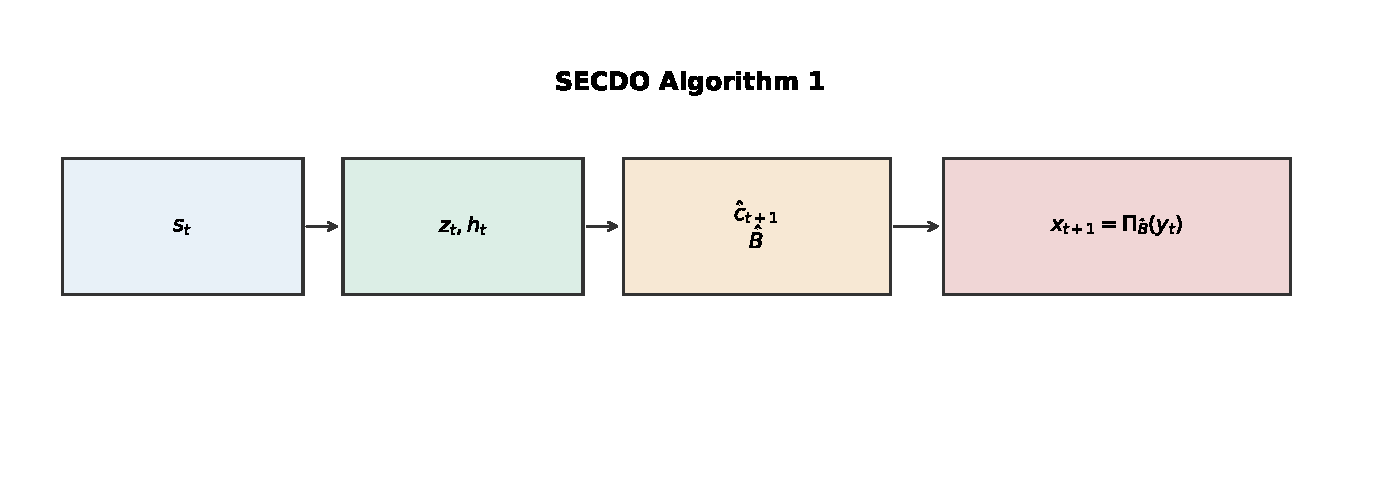
\includegraphics[width=\linewidth]{figures/fig1_framework.pdf}
\caption{SECDO loop: state encoding, constraint prediction, predictability-conditioned mixed projection.}
\label{fig:framework}
\end{figure}
